\documentclass[10pt]{article}

\usepackage{fancyhdr}
\usepackage{graphicx}
\usepackage{geometry}
\usepackage{lastpage}
\usepackage{titling}
\usepackage{sectsty}
\usepackage{setspace}
\usepackage{changepage}
\usepackage[shortlabels]{enumitem}
\usepackage{subcaption}
\usepackage{helvet}
\usepackage{hyperref}

\usepackage{tabularx}
\usepackage[table]{xcolor}
\usepackage{array}
\newcolumntype{P}[1]{>{\centering\arraybackslash}p{#1}}

\usepackage{siunitx}
\usepackage{nicefrac}
\usepackage{amsmath}
\usepackage{gensymb}
\usepackage{amssymb}
\usepackage{float}
\setcounter{MaxMatrixCols}{11}
\usepackage{indentfirst}

\usepackage{listings}
\usepackage{matlab-prettifier}
% \usepackage{color}
% \definecolor{dkgreen}{rgb}{0,0.6,0}
% \definecolor{gray}{rgb}{0.5,0.5,0.5}
% \definecolor{mauve}{rgb}{0.58,0,0.82}

\lstset
{
  frame=tb,
  style=Matlab-editor,
  % language=MATLAB, %Matlab-editor,
  aboveskip=3mm,
  belowskip=3mm,
  showstringspaces=false,
  columns=flexible,
  basicstyle={\small\ttfamily},
  numbers=none,
  % numberstyle=\tiny\color{gray},
  % keywordstyle=\color{blue},
  % commentstyle=\color{dkgreen},
  % stringstyle=\color{mauve},
  breaklines=true,
  breakatwhitespace=true,
  tabsize=3
}

\geometry
{
  letterpaper, 
  total={175.9mm,229.4mm}, 
  top=25mm, 
  left=20mm, 
  headheight=15pt,
  voffset=12pt,
  footskip=15pt
}
\author{Daniel Sturdivant}
\title{Homework 4}
\date{May 2023}
\graphicspath{ {./media/} }

\pagestyle{fancy}
\fancyhead[R]{May 2, 2023}
\fancyhead[L]{Sturdivant, Daniel}
\fancyhead[C]{MECH 7710 Optimal}
\fancyfoot[C]{Page \thepage\ of \pageref{LastPage}}

\makeatletter
\def\@maketitle
{
  \null
  \begin{center}
    {\huge \@title \\}
  \end{center}
  \vskip 5mm
}
\makeatother

\sectionfont{\fontsize{16}{16}}
\subsectionfont{\fontsize{13}{13}\normalfont}
\renewcommand{\thesubsection}{\arabic{section}-\arabic{subsection}}
\renewcommand{\familydefault}{\sfdefault}
\newcommand{\solution}{\textbf{Solution: \\}}


%% ========================================================================== %%
\begin{document}

\maketitle
\thispagestyle{fancy}
\setstretch{1.25}
% \setlength{\parskip}{0em}
% \setlength{\abovedisplayskip}{-8pt}
% \setlength{\belowdisplayskip}{12pt}
\setlength{\parindent}{0pt}

\begin{enumerate}[label=\textbf{\arabic*.}]
  \itemsep 24pt
  
  % PROBLEM 1
  \item Develop a model for a pendulum with inertia $J_p = 2.5 
  \frac{\si{Nm}}{\si{rad/s^2}}$, mass $m=1.6 \si{kg}$ and length $L = 1\si{m}$. 
  The pin introduces damping in the system that should be modeled as $T_b = b 
  \dot{\theta}^3$ where $b = 1.25 \frac{\si{Nm}}{\si{rad/s}}$. The input to the 
  system is a torque at the pin given by $T = 12 \si{Nm}$. Assume the system is 
  acted on by a horizontal disturbance force at the end of the pendulum,
  $F(t) = 5 + \eta$ where $\eta \sim N(0,2)$. The measurement of the angle of 
  the pendulum is corrupted by zero mean Gaussian white noise with variance of 1 
  degree.
  \begin{enumerate}[(a)]
    \itemsep -2pt 
    \item Develop a simulation of the system.
    \item Develop an Extended Kalman Filter to estimate the position and 
    velocity (and any additional needed parameters) of the pendulum given 
    measurement as described.
    \item Develop an Unscented Kalman Filter to estimate the position and 
    velocity (and any additional needed parameters) of the pendulum given 
    measurement as described.
    \item Use Monte Carlo simulation to compare the performance of the EKF and 
    UKF. Be sure to compare expected covariance to sampled covariance from 
    Monte Carlo simulations.
  \end{enumerate}
  \solution
  The following continuous model was designed for this system (\emph{Equation 
  \ref{eq:1}}):
  \begin{equation}
    \ddot{\theta}(t) = \dfrac{1}{J} \left(T + F(t)l\cos{(\theta(t))} - b\dot{\theta}(t)^3 - mgl\sin{(\theta(t))}\right)
    \label{eq:1}
  \end{equation}
  From this equation, both angular velocity, $\dot{\theta}$, and angle, 
  $\theta$, can be Euler integrated from $\ddot{\theta}$ as the simulated 
  system. It is easy to see that there are 3 terms that are functions of time in 
  this equation; $\theta(t)$, $\dot{\theta}(t)$, and $F(t)$. These variables 
  become the states of the Kalman Filters.

  \begin{figure}[H]
    \centering
    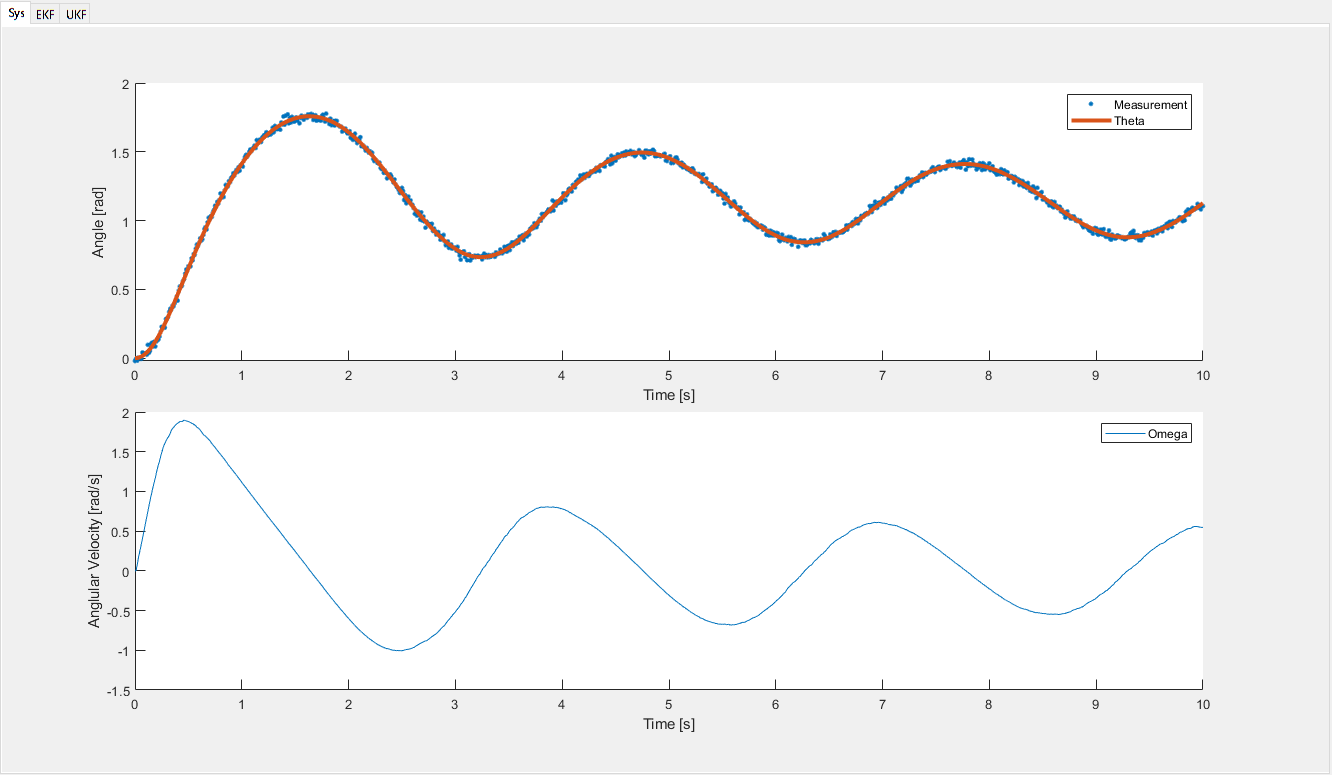
\includegraphics[width=0.7\textwidth]{p1_sys.png}
    \caption{System Simulation.}
    \label{fig:1}
  \end{figure}

  In order to create the Extended Kalman Filter, the Jacobian Matrix with 
  respect to each of the defined variables must be created. This defines the 
  state transition matrix for the system. For this system, the observation 
  matrix is directly mapped to the state of the angle, $\theta$.
  \begin{equation}
    \begin{split}
      A &= \dfrac{1}{J}
      \begin{bmatrix}
        0 & J & 0 \\ 
        -(F_{k-1}l\sin{(\theta_{k-1})} + mgl\cos{(\theta_{k-1})}) & -3b\dot{\theta}_{k-1}^2 & l\cos{(\theta_{k-1})} \\
        0 & 0 & 0
      \end{bmatrix} \\
      A_d &\approx eye(3) + A\Delta t \\
      C &= \begin{bmatrix} 1 & 0 & 0 \end{bmatrix}
    \end{split}
    \label{eq:2}
  \end{equation}

  For both the EKF and UKF, since the model is known perfectly, the process 
  noise is assumed to be small compared to the measurement noise.
  \begin{equation}
    \begin{split}
      Q &= \begin{bmatrix} 1^{-6} & 0 & 0 \\ 0 & 1^{-6} & 0 \\ 0 & 0 & 1^{-6} \end{bmatrix} \\
      R &= 1
    \end{split}
    \label{eq:3}
  \end{equation}

  A nonlinear time update along with the standard, linear Kalman measurement 
  update was used in the EKF. For this system, the Jacobian is only necessary 
  for the propagation of the covariance. The following code was used to model 
  the EKF.
  \begin{lstlisting}
  for k = 2:len
    % predict
    A = [0, ...
         1, ...  
         0; ...
         -(l*x_ekf(3,k-1)*sin(x_ekf(1,k-1)) + m*g*l*cos(x_ekf(1,k-1)))/J, ...
         -3*b*x_ekf(2,k-1)^2/J, ... 
         l*cos(x_ekf(1,k-1))/J; ...
         0, ...
         0, ...
         0];
    
    dt = t(k) - t(k-1);
    A = eye(3) + A*dt;

    alpha_ekf(k) = 1/J * (T + x_ekf(3,k-1)*l*cos(x_ekf(1,k-1)) - b*x_ekf(2,k-1)^3 - m*g*l*sin(x_ekf(1,k-1)));
    x_ekf(1,k) = wrapToPi(x_ekf(1,k-1) + x_ekf(2,k-1)*dt + 0.5*alpha_ekf(k)*dt^2);
    x_ekf(2,k) = x_ekf(2,k-1) + alpha_ekf(k)*dt;
    x_ekf(3,k) = x_ekf(3,k-1);
    P(:,:,k) = A*P(:,:,k-1)*A' + Q;

    % correct
    C = [1, 0, 0];
    L = P(:,:,k)*C'*(C*P(:,:,k)*C' + R)^-1;
    P(:,:,k) = (eye(3) - L*C) * P(:,:,k);
    x_ekf(:,k) = x_ekf(:,k) + L*(y(k) - C*x_ekf(:,k));
  end
  \end{lstlisting}

  This results in \emph{Figure \ref{fig:2}}.

  \begin{figure}[H]
    \centering
    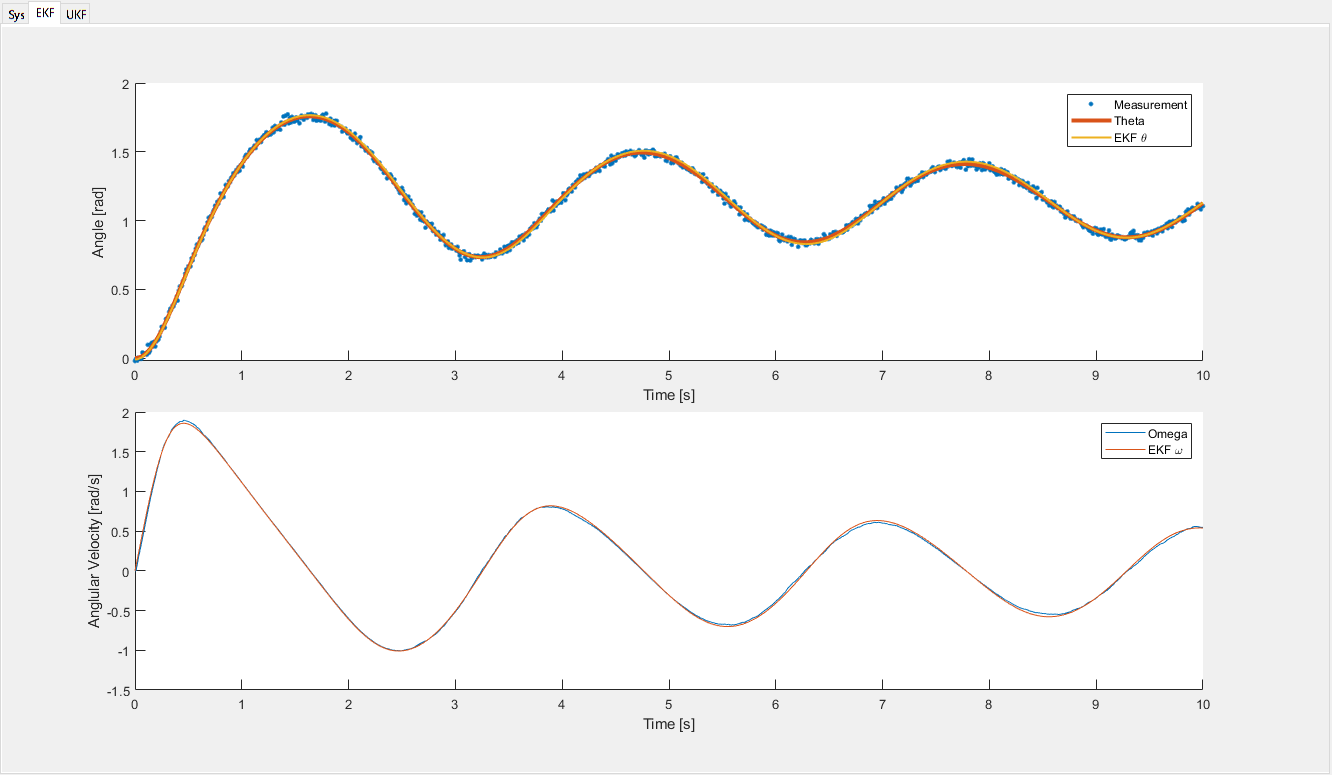
\includegraphics[width=0.75\textwidth]{p1_ekf.png}
    \caption{Extended Kalman Filter.}
    \label{fig:2}
  \end{figure}

  The creation of the Unscented Kalman Filter requires the use of the Unscented 
  Transform which is more complex than linearizing a system. Both the time and 
  measurement updates are broken down in two distinct parts as described below:
  \begin{equation}
    \begin{split}
      &\text{\textbf{Time Update 1/2: Create Sigma Points and Weights}} \\
      &X_0^{(\sigma)} = \hat{x}_{k-1}^+ \\
      &W_0^{m} = \dfrac{\lambda}{n + \lambda} \\
      &W_0^{c} = \dfrac{\lambda}{n + \lambda} + (1 - \alpha^2 + \beta) \\
      &X_i^{(\sigma)} = \hat{x}_{k-1}^+ + \left(\sqrt{(n+\lambda)P_{k-1}^+}\right)_i \:\text{ $\forall$ $i=1...n$} \\
      &X_i^{(\sigma)} = \hat{x}_{k-1}^+ - \left(\sqrt{(n+\lambda)P_{k-1}^+}\right)_{i-n} \:\text{ $\forall$ $i=n+1...2n$} \\
      &W_i^{m} = W_i^{c} = \dfrac{\lambda}{2(n + \lambda)} \:\text{ $\forall$ $i=1...2n$} \\
      &\text{\textbf{Time Update 2/2: Propagate State Mean and Covariance}} \\
      &X_i^{(\sigma)} = f(X_i^{(\sigma)}, Q) \\
      &\hat{x}_k^- = \sum_{i=0}^{2n} W_i^{m}X_i^{(\sigma)} \\
      &Y_i^{(\sigma)} = h(X_i^{(\sigma)}, R) \\
      &\hat{y}_k = \sum_{i=0}^{2n} W_i^{m}Y_i^{(\sigma)} \\
      &P_k^- = \sum_{i=0}^{2n}  W_i^{c} (X_i^{(\sigma)}-\hat{x}_k^-)(X_i^{(\sigma)}-\hat{x}_k^-)^T \\
      &\text{\textbf{Measurement Update 1/2: Extrapolate Covariance}} \\
      &P_{\hat{y}_{k}\hat{y}_{k}} = \sum_{i=0}^{2n}  W_i^{c} (Y_i^{(\sigma)}-\hat{y}_k)(Y_i^{(\sigma)}-\hat{y}_k)^T \\
      &P_{\hat{x}_{k}^-\hat{y}_{k}} = \sum_{i=0}^{2n}  W_i^{c} (X_i^{(\sigma)}-\hat{x}_k^-)(Y_i^{(\sigma)}-\hat{y}_k)^T \\
      &\text{\textbf{Measurement Update 1/2: Correct State and Covariance}} \\
      &L_k = P_{\hat{x}_{k}^-\hat{y}_{k}} P_{\hat{y}_{k}\hat{y}_{k}}^{-1} \\
      &P_k^+ = P_k^- - L_k P_{\hat{y}_{k}\hat{y}_{k}} L_k^T \\
      &\hat{x}_k^+ = \hat{x}_k^- + L_k(y_k - \hat{y}_k)
    \end{split}
    \label{eq:4}
  \end{equation}
  Where $\lambda=\alpha^2(n+\kappa) - n$ is the scaling parameter defined by 
  $\alpha=1^{-3}$, $\beta=2$, and $\kappa=0$. $W_i^{m}$ is the measurement 
  weight and $W_i^{c}$ is the covariance weight. $(\sqrt{(n+\lambda)P_{k-1}^+})_i$ 
  is the \emph{i-th} column vector of the matrix square root. The following is 
  code for the UKF assuming the same $Q$ and $R$ as the EKF.
  \begin{lstlisting}
  for k = 2:len
    dt = t(k) - t(k-1);

    % square root of covariance
    P_sqrt = chol((n + lambda) * P_ukf(:,:,k-1));
    Pxy = zeros(n,1);
    Pyy = 0;

    % first sigma point
    sig(:,1) = x_ukf(:,k-1);
    Wm(1) = lambda / (n + lambda);
    Wc(1) = Wm(1) + (1 - alpha^2 + beta);

    alpha_ukf(1,k) = 1/J * (T + sig(3,1)*l*cos(sig(1,1)) - b*sig(2,1)^3 - m*g*l*sin(sig(1,1)));
    xHat(1,1) = wrapToPi(sig(1,1) + sig(2,1)*dt + 0.5*alpha_ukf(1,k)*dt^2);
    xHat(2,1) = sig(2,1) + alpha_ukf(1,k) * dt;
    xHat(3,1) = sig(3,1);

    yHat(1) = C * xHat(:,1);
    x_ukf(:,k) = x_ukf(:,k) + Wm(1) * xHat(:,1);
    y_ukf(k) = y_ukf(k) + Wm(1) * yHat(1);

    for i = 1:2*n
        % sigma points
        if i < 4
            sig(:,i+1) = sig(:,1) + P_sqrt(:,i);
        else
            sig(:,i+1) = sig(:,1) - P_sqrt(:,i-n);
        end
        Wm(i+1) = 1 / (2*(n+lambda));
        Wc(i+1) = Wm(i+1);

        % propogated sigma point mean
        alpha_ukf(i+1,k) = 1/J * (T + sig(3,i+1)*l*cos(sig(1,i+1)) - b*sig(2,i+1)^3 - m*g*l*sin(sig(1,i+1)));
        xHat(1,i+1) = wrapToPi(sig(1,i+1) + sig(2,i+1)*dt + 0.5*alpha_ukf(i+1,k)*dt^2);
        xHat(2,i+1) = sig(2,i+1) + alpha_ukf(i+1,k) * dt;
        xHat(3,i+1) = sig(3,i+1);
        x_ukf(:,k) = x_ukf(:,k) + Wm(i+1) * xHat(:,i+1);

        % propagated sigma point measurement mean
        yHat(i+1) = C * xHat(:,i+1);
        y_ukf(k) = y_ukf(k) + Wm(i+1) * yHat(i+1);
    end

    % propogated system covariance
    for i = 1:(2*n + 1)
        P_ukf(:,:,k) = P_ukf(:,:,k) + Wc(i) * ( (xHat(:,i)-x_ukf(:,k)) * (xHat(:,i)-x_ukf(:,k))' );
        Pyy = Pyy + Wc(i) * ( (yHat(i)-y_ukf(k)) * (yHat(i)-y_ukf(k))' );
        Pxy = Pxy + Wc(i) * ( (xHat(:,i)-x_ukf(:,k)) * (yHat(i)-y_ukf(k))' );
    end
    Pyy = Pyy + R;
    P_ukf(:,:,k) = P_ukf(:,:,k) + Q;

    % correction
    L = Pxy * Pyy^-1;
    P_ukf(:,:,k) = P_ukf(:,:,k) - L*Pyy*L';
    x_ukf(:,k) = x_ukf(:,k) + L*(y(k) - y_ukf(k));

  end
  \end{lstlisting}

  This results in \emph{Figure \ref{fig:3}}.

  \begin{figure}[H]
    \centering
    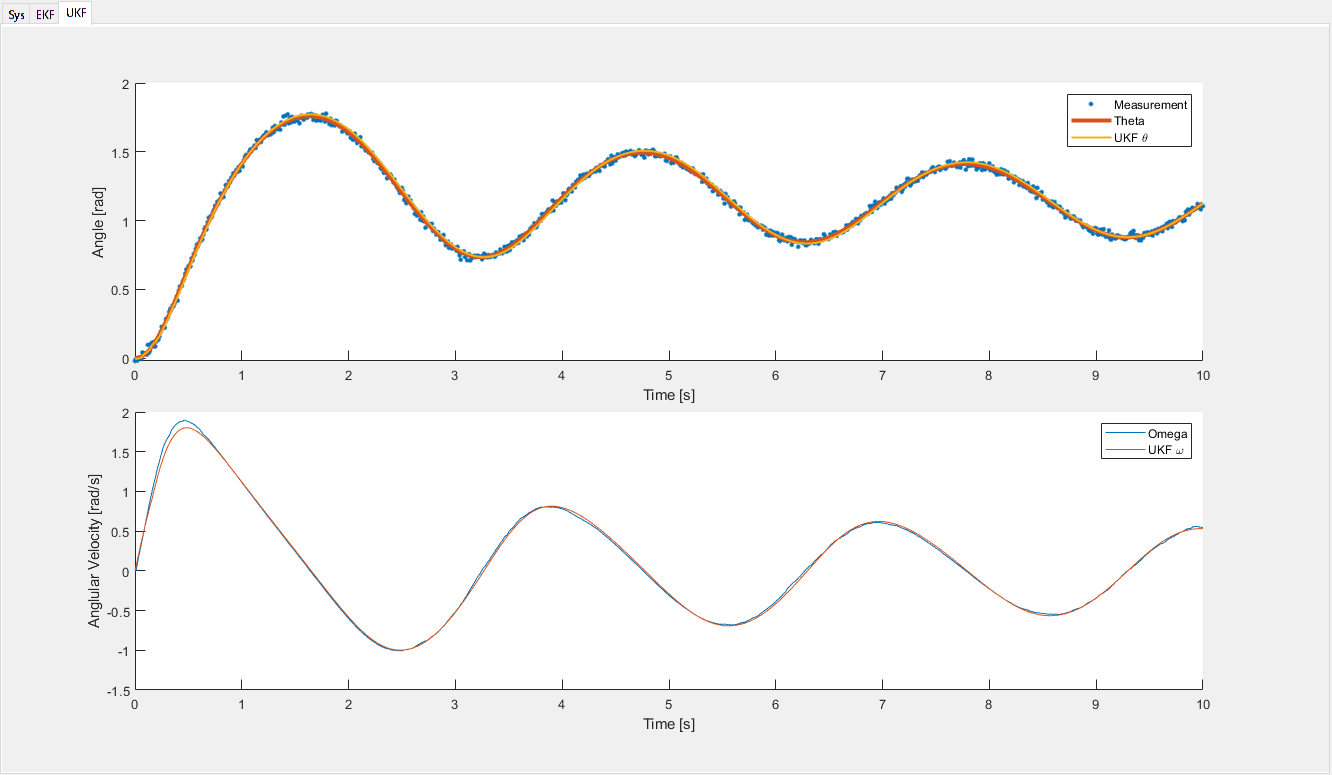
\includegraphics[width=0.75\textwidth]{p1_ukf.png}
    \caption{Unscented Kalman Filter.}
    \label{fig:3}
  \end{figure}

  No monte carlo analysis was performed but the actual performance of the EKF 
  and UKF on this system is almost identical using the specified parameters.

  \vspace{24pt}

  % PROBLEM 2
  \item Repeat problem 4 from HW2. Convince yourself that the Least Squares 
  solution you developed is the same as the solution given from \emph{arx.m}. 
  What are the ARX inputs to recover the least squares solution you developed 
  in HW2.
  \begin{enumerate}[(a)]
    \item Now crank up the sensor noise to $\sigma=1.0$. Try using higher order 
    ARX fits. Can you identify the model?
    \item What about with another model form? Which model form worked best? How 
    good is the fit (provide plots for proof)? What was the order of the fit?
  \end{enumerate}
  \solution
  For the second order system, using \emph{arx([Y U], [2 2 1])} results in the 
  same solution as using least squares.
  \begin{figure}[H]
    \centering
    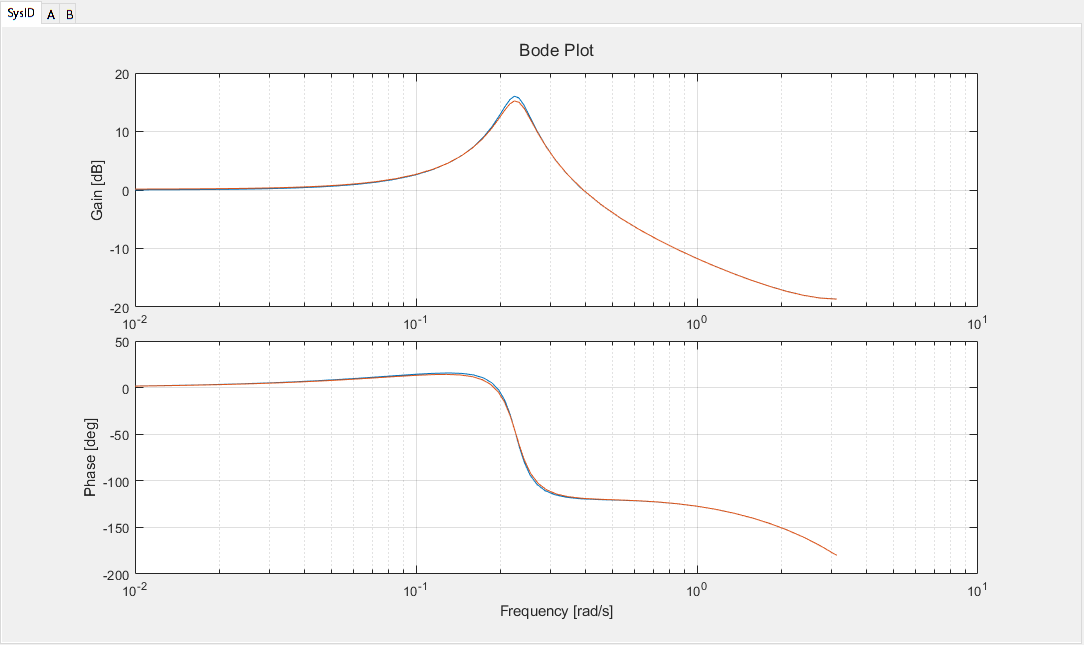
\includegraphics[width=0.75\textwidth]{p2_sysid.png}
    \caption{SysID with $\sigma=0.1$.}
    \label{fig:4}
  \end{figure}
  When changing the noise to 1, a much higher order system was needed to emulate 
  the correct response. \emph{arx([Y U], [11 11 1])} was found to provide a 
  close approximation.
  \begin{figure}[H]
    \centering
    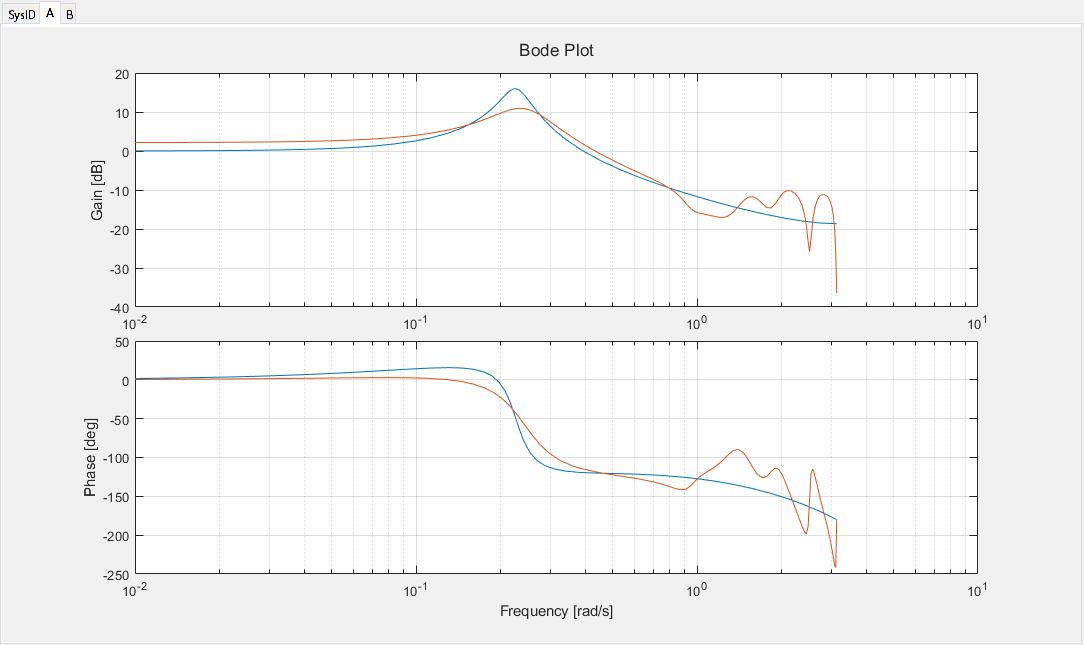
\includegraphics[width=0.75\textwidth]{p2_a.png}
    \caption{SysID with $\sigma=1.0$.}
    \label{fig:5}
  \end{figure}

\end{enumerate} 

\end{document}